\section{概要设计}

\subsection{大雾实验工具}

\subsubsection{总体功能说明}

本工具通过腾讯云服务器搭建于网页平台,支持任何设备自由访问。
传入实验数据后,本工具立刻完成绘制图像、计算不确定度、生成计算公式等一系列操作,
并将最终结果整理成一份 Word 文档,下载后即可直接使用。
本实验工具支持大学物理-基础实验的 49 个实验,这大大提升了学生们撰写实验报告的效率。
由于本工具只是将传入的实验数据进行自动分析,故其不会造成抄袭、造假等学术不端问题。

\subsubsection{具体功能点说明}

使用本工具时,用户只需输入他们做实验时测量到的原始数据,
而无需任何额外的计算处理,用户所要做的只有按照规定的格式上传 Excel 文档。
本工具支持 \verb|xlsx|, \verb|csv| 等各种格式的数据表格。
具体而言,每个实验都会有一张示例数据表供用户参考,如图 \ref{fig:interface} 的界面所示。
用户也可以直接下载示例数据,并直接在它的基础上进行修改。
因此,本工具没有任何学习成本,是一款即点即用、免安装的简单轻应用。

\begin{figure}[p]
  \centering
  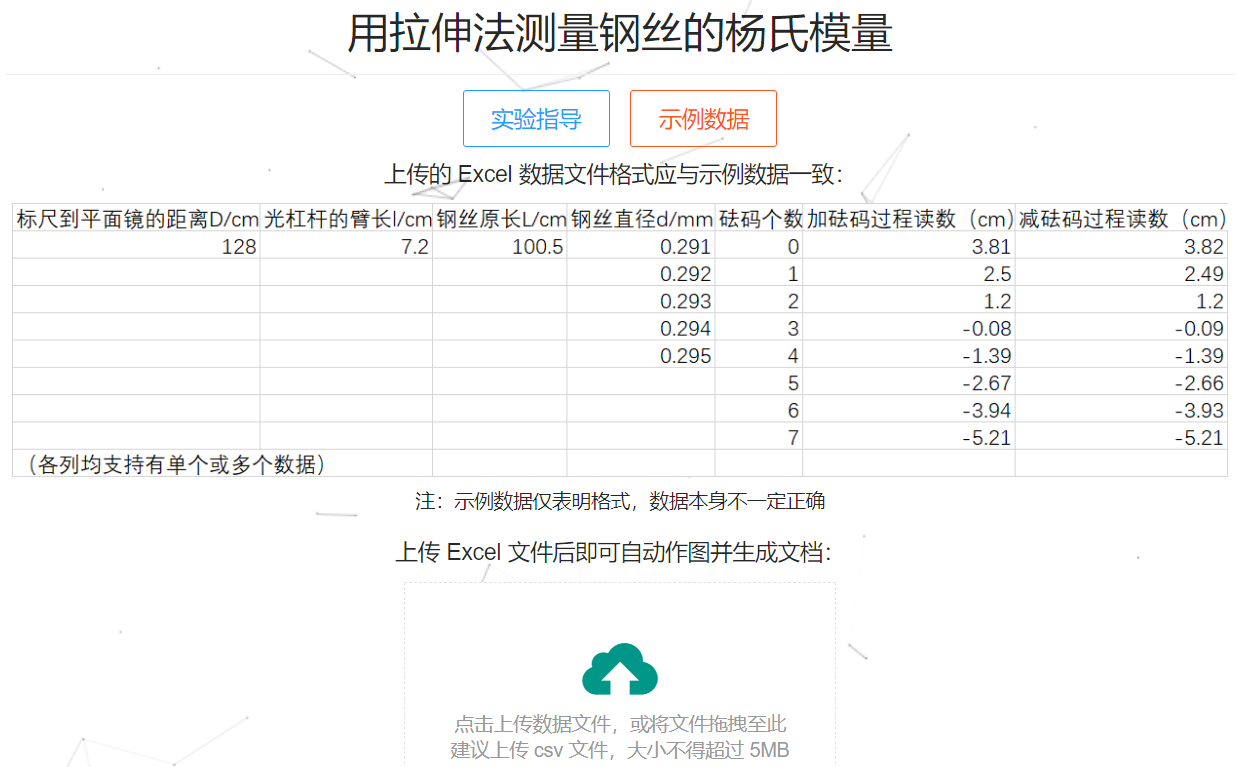
\includegraphics[width=0.67\columnwidth]{figure/interface.png}
  \caption{“拉伸法测钢丝杨氏模量”的工具界面}
  \label{fig:interface}
\end{figure}

另外,本工具贴心地提供了不确定度表格与通用的计算工具,并且每个实验都附有可在线浏览的实验指导。

{\noindent\bfseries\textbullet{}绘制图像}

本工具根据输入的数据以及实验原理,自动生成美观的实验图像,
支持平滑去噪、数据拟合、双 y 图等多种图像生成需求,如图 \ref{fig:draw} 所示。

\begin{figure}[p]
  \centering
  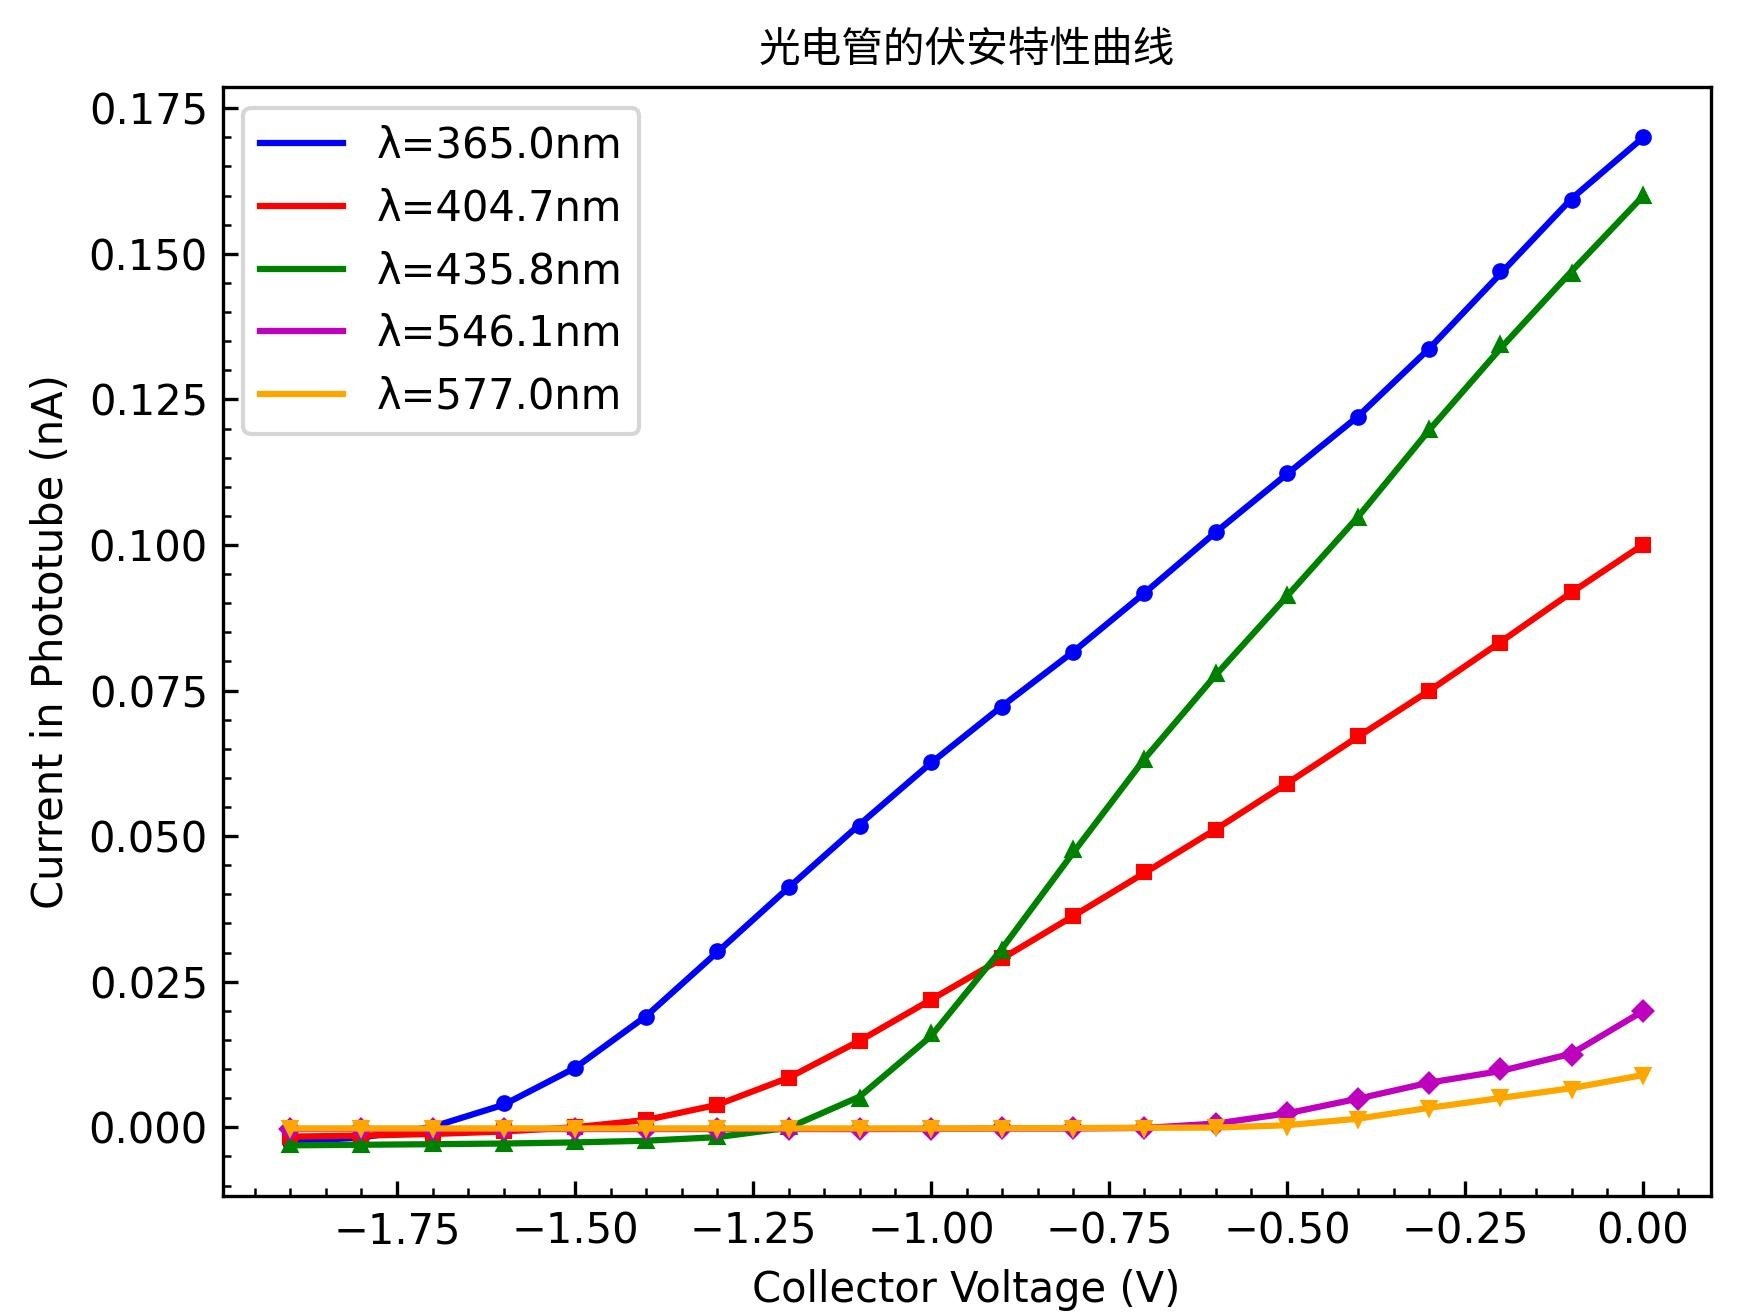
\includegraphics[width=0.67\columnwidth]{figure/draw.jpg}
  \caption{平滑连接的光电效应伏安特性曲线}
  \label{fig:draw}
\end{figure}

{\noindent\bfseries\textbullet{}计算不确定度与生成计算公式}

本工具在生成的 Word 文档中渲染了各种公式,如图 \ref{fig:calc} 所示。
用户可以直观看到不确定度每一步的计算过程,并在自己的报告中直接使用这些算式与结果。

\begin{figure}[p]
  \centering
  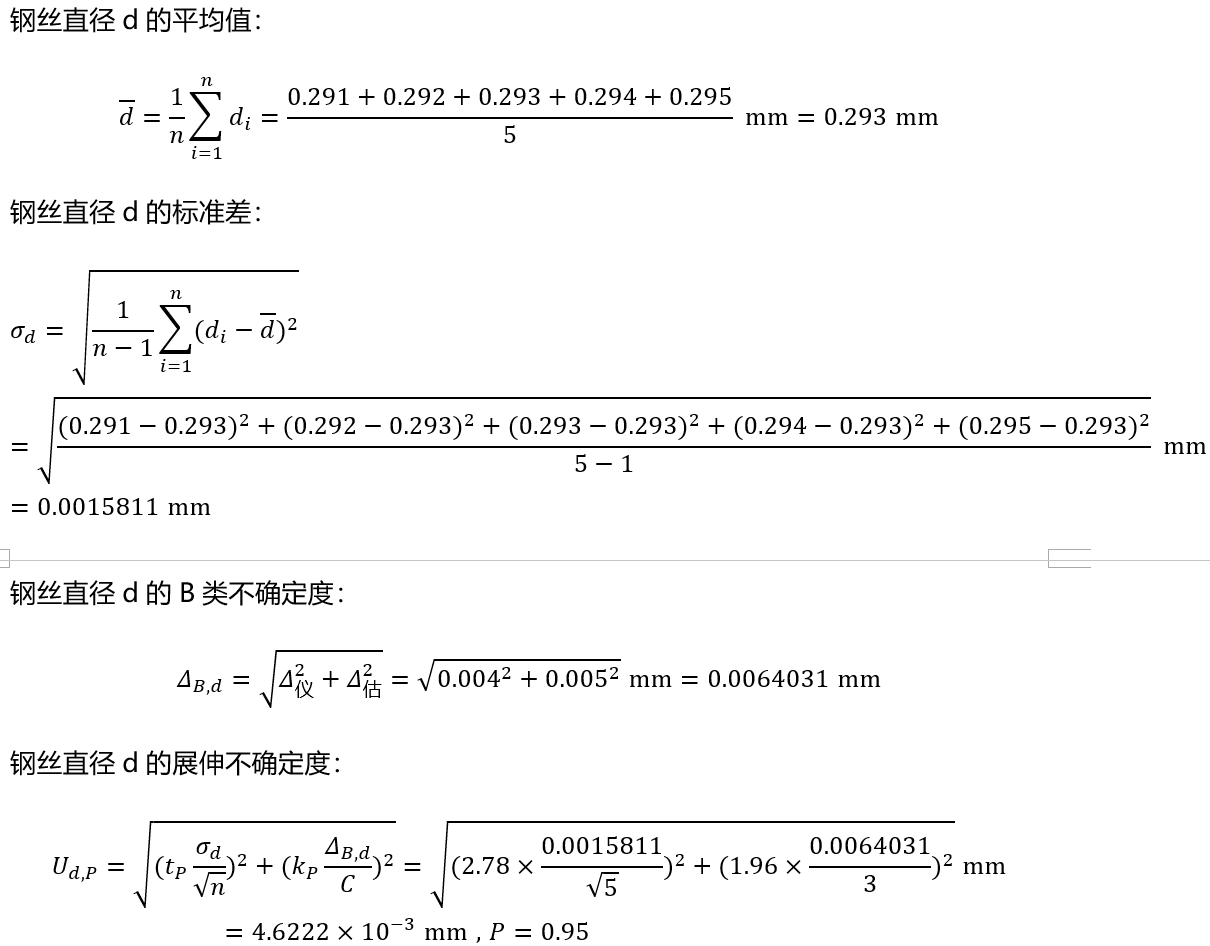
\includegraphics[width=0.67\columnwidth]{figure/calc.png}
  \caption{不确定度计算的详细过程}
  \label{fig:calc}
\end{figure}

在 Word 文档中除了有已经渲染好的公式外,
我们还提供了它们的 \LaTeX{} 源码,如图 \ref{fig:latex} 所示。
这极大方便了用 \LaTeX{}, Markdown 等排版实验报告的用户,使他们无需手动敲入每一个算式。

\begin{figure}[htbp]
  \centering
  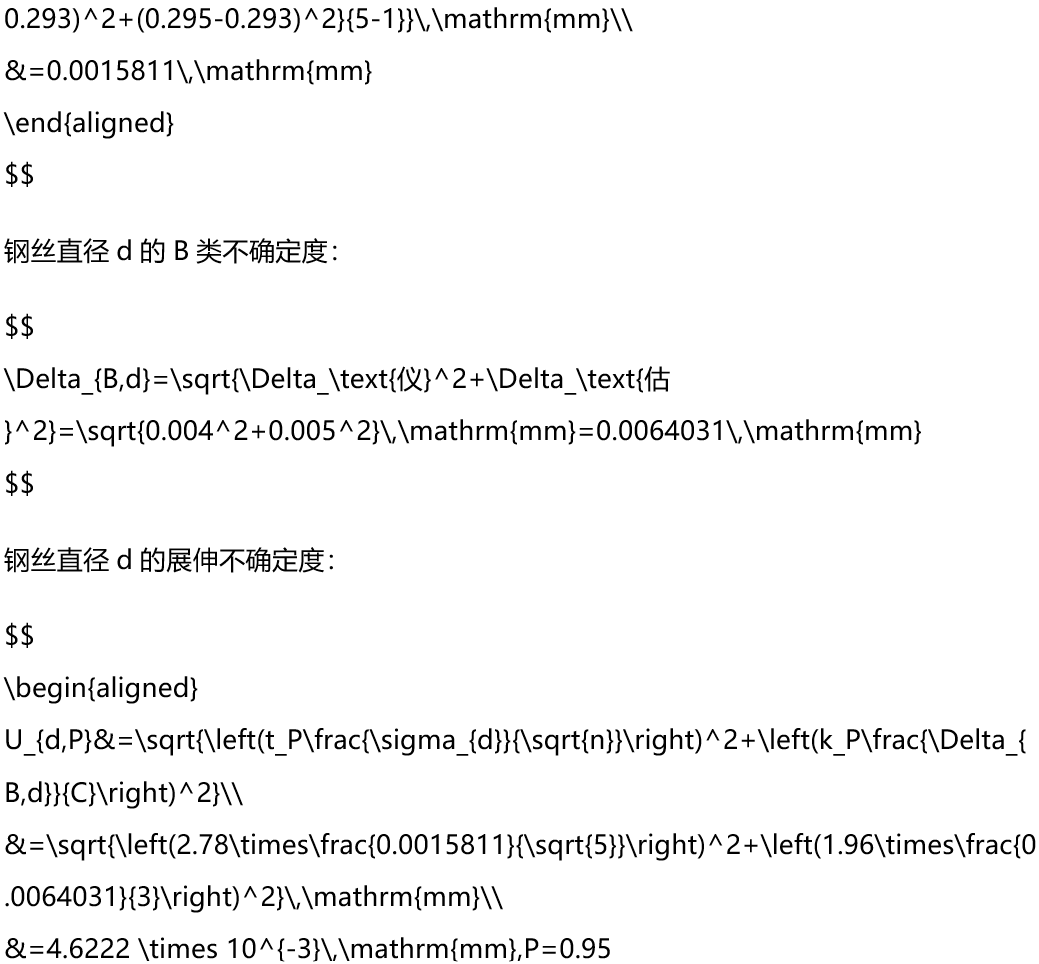
\includegraphics[width=0.67\columnwidth]{figure/latex.png}
  \caption{不确定度算式的 \LaTeX{} 源码}
  \label{fig:latex}
\end{figure}

\subsubsection{功能点设计细节}

本工具后端使用 Python 编写,使用的包与模块如表 \ref{tab:pkg} 所示。
前端由 HTML 编写,并使用了 \verb|Flask| Web 应用框架。

\begin{table}[htbp]
  \caption{本工具使用的全部 Python 包与模块}
  \label{tab:pkg}
  \vskip 0.1in
  \centering\small
  \begin{tabular}{lc}
  \toprule
  Python 包或模块 & 用途 \\
  \midrule
  \verb|chardet| & 检测用户上传的数据表格的编码 \\
  \verb|collections| & 通过 \verb|namedtuple| 使代码更清晰 \\
  \verb|Flask| & Web 应用框架 \\
  \verb|latex2mathml| & \LaTeX{} 代码转换为 \verb|MathML| 代码 \\
  \verb|lxml| & \verb|MathML| 代码转 \verb|Office MathML| \\
  \verb|math|, \verb|numpy| & 不确定度数字运算 \\
  \verb|Matplotlib| & 绘制物理图像 \\
  \verb|os|, \verb|random|, \verb|shutil| & 后台文件操作与管理 \\
  \verb|pandas| & 数据表格处理 \\
  \verb|python-docx| & 生成 Word 文档 \\
  \verb|SciPy| & 数据拟合 \\
  \verb|SymPy| & 不确定度符号运算 \\
  \verb|time|, \verb|threading| & 定时删除生成的 Word 文档 \\
  \verb|traceback| & 打印运行错误以便调试 \\
  \bottomrule
  \end{tabular}
  \vskip -0.1in
\end{table}

关于图像绘制、数据处理、文档生成的具体规范和接口可参见\href{https://github.com/feixukeji/PhyX/blob/main/README.md}{{开发说明}}、\href{https://github.com/feixukeji/PhyX/blob/main/%E6%95%B0%E6%8D%AE%E5%A4%84%E7%90%86API%E6%8C%87%E5%8D%97.md}{{数据处理API指南}}、\href{https://github.com/feixukeji/PhyX/blob/main/%E5%85%AC%E5%BC%8F%E6%8F%92%E5%85%A5API%E6%8C%87%E5%8D%97.md}{{公式插入API指南}}。

\subsubsection{性能和效率}

尽管工具实现的任务非常复杂,但它仍然能够在 1 秒内根据用户上传的数据生成文档,可见性能之卓越。

\subsection{蜗壳排课工具}

\subsubsection{总体功能说明}

该工具是一个网页应用,使用方便快捷。在主页面,已添加的课程列表会被清晰地展示出来,用户可以通过点击“添加课程”、“编辑课程”或“开始排课”,进入相应的界面,如图 \ref{fig:p1} 所示。

\begin{figure}[htbp]
  \centering
  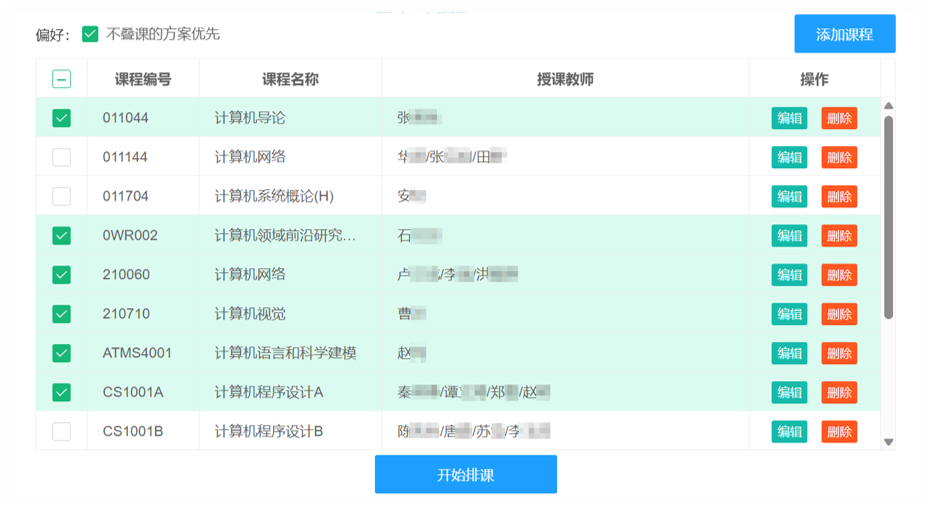
\includegraphics[width=\columnwidth]{figure/p1.png}
  \caption{蜗壳排课工具主页}
  \label{fig:p1}
\end{figure}

图 \ref{fig:p2} 展示了本工具的“添加课程”页面。在此页面,用户可以通过各种信息,如课程编号、课程名称、教师名称等进行课程搜索,我们的网站已经收录了超过 2500 个课程,并会定期从教务系统自动更新。

课程列表呈现了课程名称、授课教师、时间地点等信息。此外,我们还引入了评课社区的课程评级,供用户参考。在添加课程时,用户可以为每个课程设定一个喜好程度,然后工具会根据这个喜好程度和课程时间自动进行课程安排。

\begin{figure}[htbp]
  \centering
  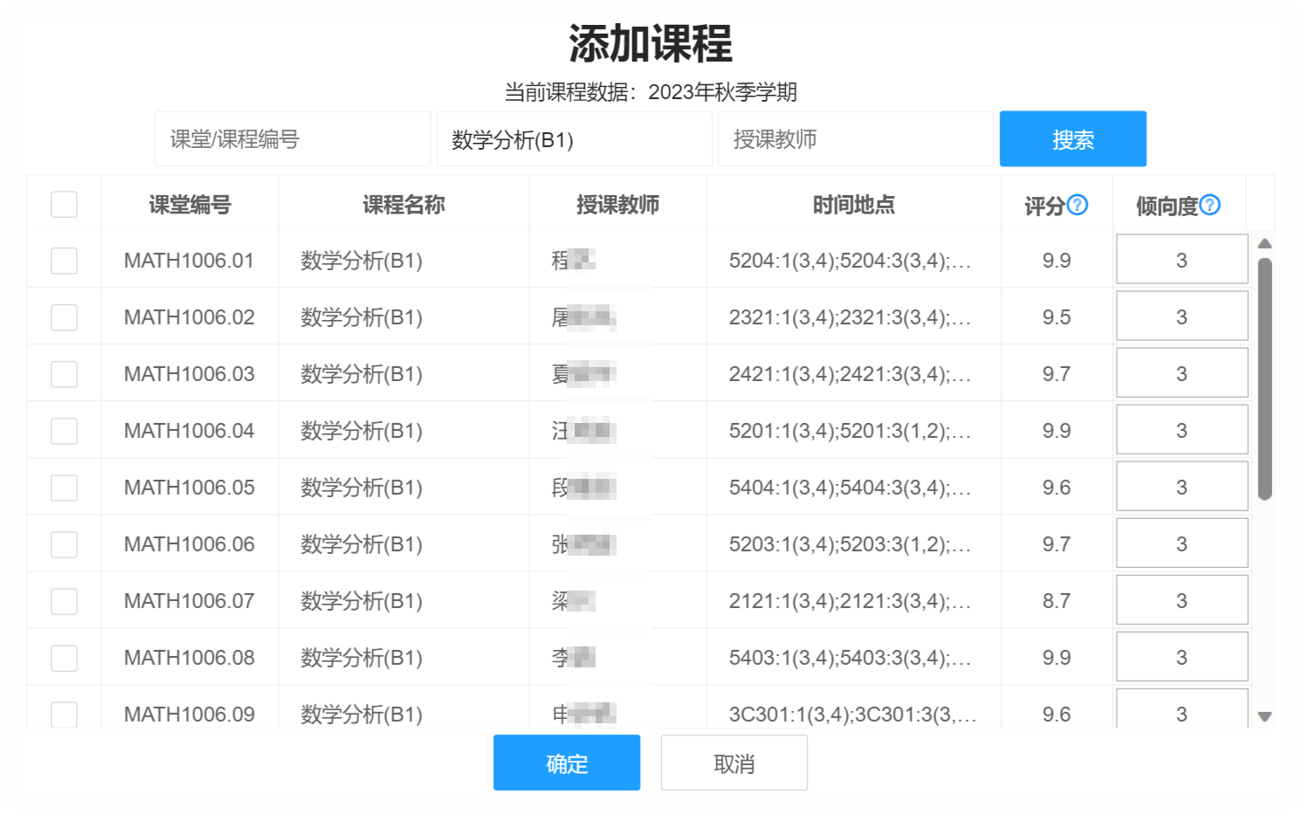
\includegraphics[width=\columnwidth]{figure/p2.png}
  \caption{蜗壳排课工具“添加课程”页面}
  \label{fig:p2}
\end{figure}

\subsubsection{附加功能}

值得一提的是,在主页面可以选择偏好设置——“不叠课的方案优先”。若勾选之,则我们的排课算法优先推荐没有任何时间冲突的方案;若不勾选,则优先满足喜好程度总和最大,其次再满足“尽量不叠课”的要求。

\subsubsection{人机交互}

蜗壳排课工具做了许多的人性化处理,例如:若用户选择的通识课超过2门,这种情况违背了教务系统的选课规则,则我们会提醒用户“你选择的通识课超过2门,是否需要根据倾向度及与其他课程的冲突情况自动选择合适的2门?”;又如若用户选择课程过多,则工具会警告用户。

我们的工具提供的课程排列方案,既包括明确的列表形式,也包括直观的课程表形式。虽然课程表的样式与教务系统的基本一致,但我们对其样式做了优化,让它看起来更为清楚易懂,同时对小屏幕设备的兼容性也做了提升。

\subsubsection{性能和效率}

本工具使用深度优先搜索技术,结合大量的剪枝与智能优化,使得在用户点击“开始排课”后,在 1 秒钟之内呈现排课方案。而且,能够呈现 5 种备选方案供用户选择。

\subsubsection{隐私安全}

我们深切理解用户隐私的重要性。因此,排课算法完全在本地通过 JavaScript 运行,任何信息都不会被上传到服务器。用户可以借助 Microsoft Edge 浏览器将本站点作为应用安装,一旦安装完成,即使断网也可以正常使用。或者,也可以打开网站后,断开网络,仍然能够实现排课,可见算法确实在本地运行。

\subsection{我的科大APP}

\subsubsection{总体功能说明}

我的科大APP提供了包括教室查询、学校周边、校园导航等在内的 34 项链接功能,还有任务清单、资料分享等 7 项我们自主研发的功能,如图 \ref{fig:m1} 所示。而软件安装包仅有 \qty{2.5}{\mega\byte},安装后体积也仅 \qty{5}{\mega\byte},可以说是十分小巧却功能全面。

\begin{figure}[htb]
  \centering
  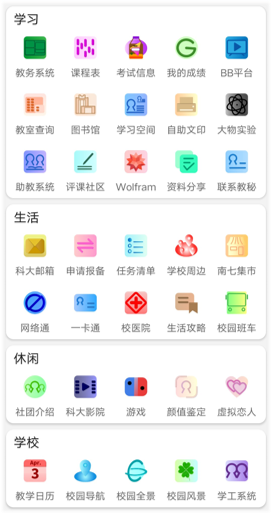
\includegraphics[width=0.6\columnwidth]{figure/m1.png}
  \caption{我的科大APP功能示意}
  \label{fig:m1}
\end{figure}

本项目主要使用 Android Studio 开发工具,结合了 Kotlin 和 HTML, JavaScript, CSS 等多种语言进行开发,可以在 Android 和 HarmonyOS 系统上运行。

\subsubsection{具体功能点说明}

我的科大APP拥有众多实用功能,这极大的便利了同学们的校内外生活。

\begin{enumerate}
  \item 教务系统、科大邮箱:首次打开弹出“输入账号密码”对话框,并将数据加密保存至本地,之后每次打开将自动登录。
  \item 课程表、考试信息:自动同步教务系统数据,若有更新,则会提醒用户。
  \item 学校周边:采用高德地图API,在地图上呈现周边美食、景点、休闲娱乐、超市、商城、药店、通讯、邮政、银行、酒店多种设施,方便用户快速寻找。
  \item 生活攻略、社团介绍、校园风景:使用 HTML 制作网页,APP打开对应网页,其中社团介绍可长按复制QQ群号,校园风景页面每次随机显示一张图片,根据用户投稿不定期更新。
  \item 习题分享:包含部分历年真题。
  \item 任务清单:用户可以添加、删除、编辑任务,任务可以设置标题、详细内容、日期时间,还能在完成之后打钩。
\end{enumerate}

\subsubsection{附加功能}

我的科大APP还有许多附加功能,进一步优化用户体验。

\begin{enumerate}
  \item 支持本科生和研究生用户,其中对本科生用户的功能支持更为丰富。
  \item “功能”页面分类显示,且根据用户的使用次数,在首页显示常用功能。
  \item 首页具有签到功能,签到后会显示今日运势,作为消遣使用。
  \item 支持自定义背景图片,个性化选择两种图标模式。
  \item 支持深色模式、横屏模式、分屏模式。
\end{enumerate}

\subsubsection{安全性}

为了实现自动登录统一身份认证和科大邮箱,我的科大APP将密码加密存至本地,即便手机中潜藏病毒软件,也难以窃取信息,可谓“一夫当关,万夫莫开”。

除了用于统计用户量、启动次数、版本分布等而收集的去敏化的设备信息外,我们没有将任何用户信息上传至服务器。即便如此,我们仍编写了\href{https://myustc.feixu.site/page/PrivacyPolicy.html}{{APP隐私政策}},APP将严格按照该隐私政策保护用户的信息。

软件已完成了工信部 ICP 备案并放置备案号。据我们了解,市场上的软件目前几乎均未放置备案号,在这一点上,我的科大APP遥遥领先。

此外,我的科大APP基于 Kotlin 语言开发,它是一门具有朝气和活力的语言。在 Google I/O 2017 中,Google 宣布 Kotlin 成为 Android 官方开发语言。2019 年其成为 Android 第一开发语言。相比于 Java,它引入了空安全特性,使软件更加安全。

\subsubsection{人机交互}

我的科大APP在图标、文本布局、气泡提示、按钮位置等方面,经过我们的反复修改与琢磨,遵循了人体工程学的设计原则。

以功能图标为例,我们APP的图标历经 4 代变迁,首先是风格不一致的初代图标;随后统一了风格,是简约图标;再后来我们自主设计,使图标变得更为精致;最后我们采取了绚丽的拟物风图标。

在功能上,我们做了许多的人性化处理,例如:当用户在本科生模式下输入研究生学号时,APP会自动判断,并提示是否要切换为研究生模式。

再举一个细节设计的例子:在用户初次登录邮箱时,为了方便用户,APP预先在邮箱地址中添加了“@mail.ustc.edu.cn”,以防止用户——特别是新生——遗漏或忘记输入“mail.”。当然,在之后的每次登录中,账号和密码都会自动填写。这些细节的精雕细琢,都为用户带来了极致的体验。

\subsubsection{性能和效率}

我的科大APP完全没有卡顿,运行十分流畅,为用户带来极佳的使用体验。

\subsubsection{用户至上}

我们始终倾听用户的声音。一方面,APP中设有反馈选项,用户可以通过填写问卷向我们反馈;另一方面,我们还通过用户交流群发布群投票,以不断优化我们的产品。

我们采纳了用户的许多有益建议,例如实现了网页内文件下载功能,添加了“科大影院”功能,课程表添加了自定义课程的功能,实现了课程表和考试信息的自动同步,以及新课程出分时的卡片提醒。